\documentclass{article}

\usepackage{pdfpages}

\usepackage[hidelinks]{hyperref}

\usepackage{array}
\usepackage{tabularx}

\usepackage{comment}

\usepackage{tcolorbox}

\usepackage{graphicx}
\usepackage{subcaption}

\usepackage{amsmath}

\usepackage{float}

\usepackage[export]{adjustbox}

\usepackage[margin=1.25in]{geometry}

\newtcbox{\inlinecode}{on line, boxrule=0pt, boxsep=0pt, top=2pt, left=2pt, bottom=2pt, right=2pt, colback=gray!15, colframe=white, fontupper={\ttfamily \footnotesize}}

\begin{document}
\pagenumbering{gobble}

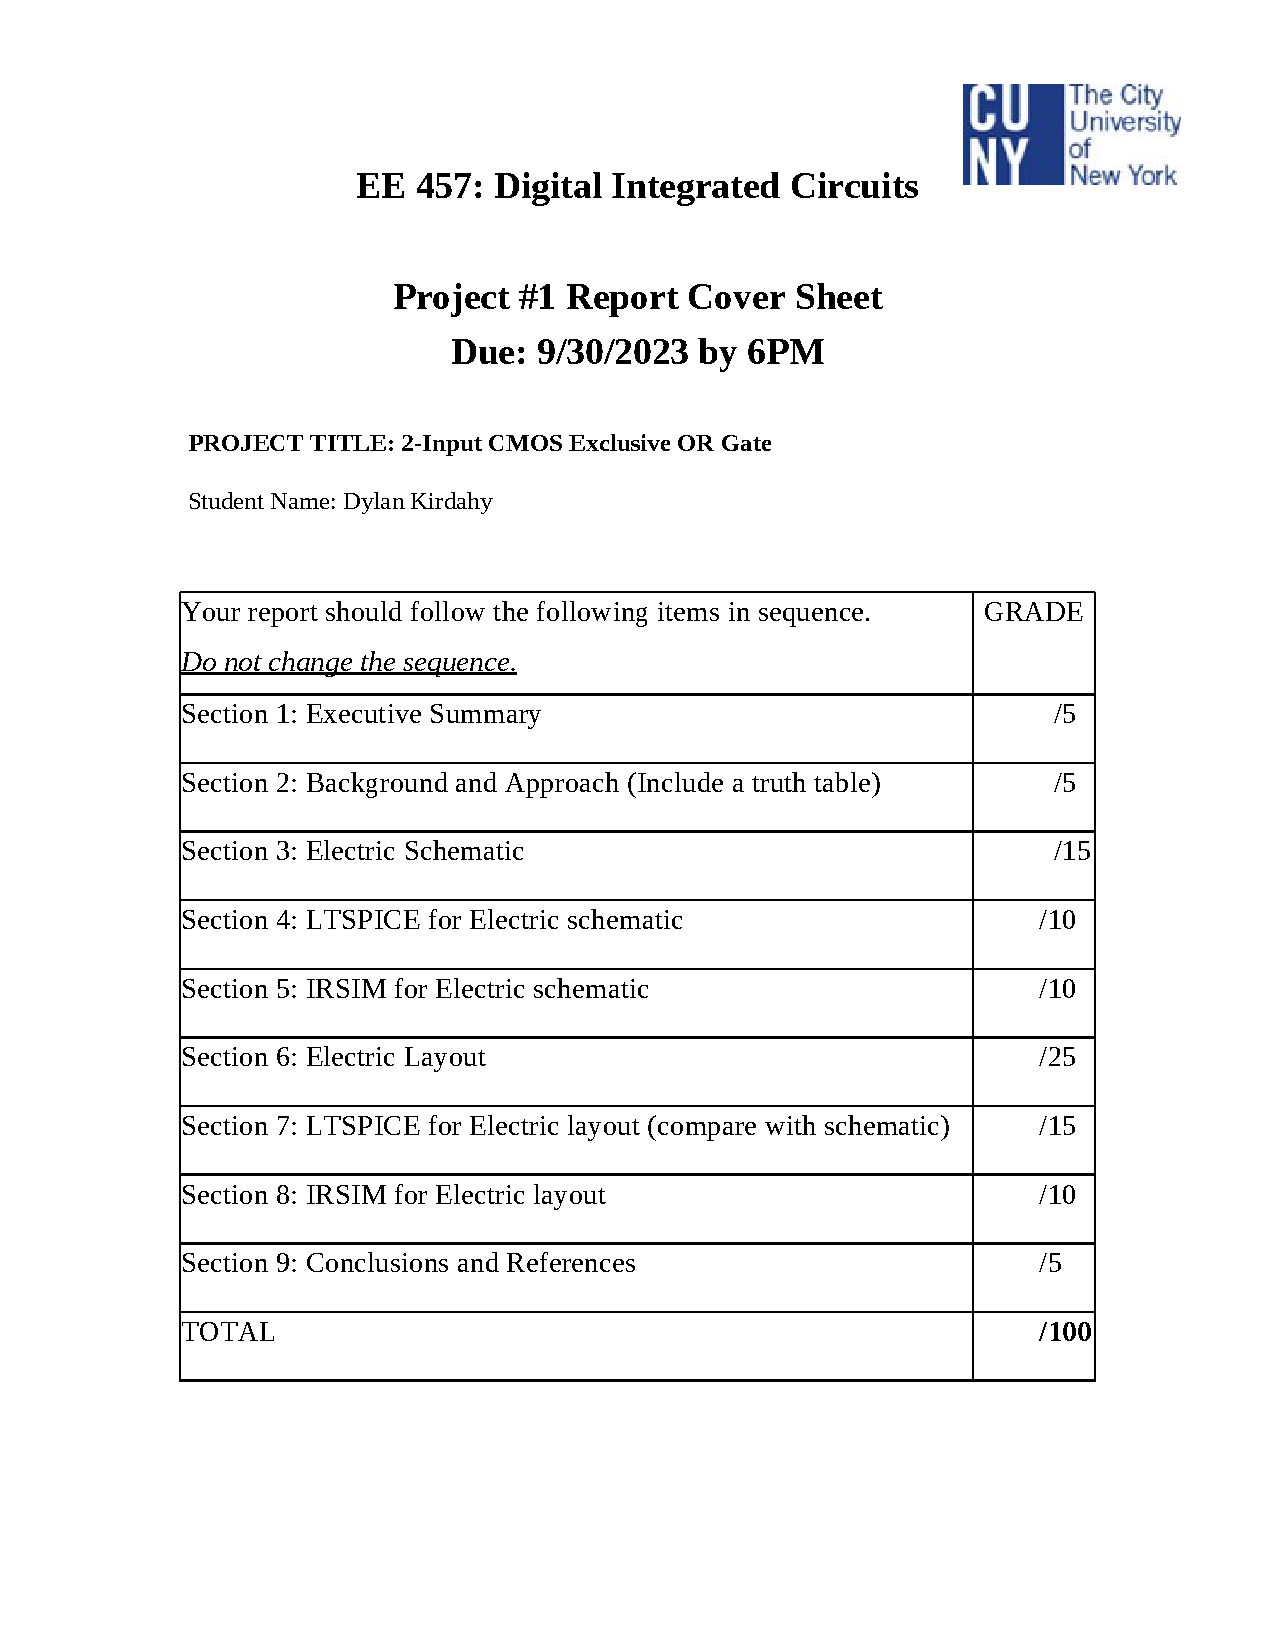
\includepdf[pages=-,scale=1,pagecommand={}]{project-1-cover-sheet.pdf}

\tableofcontents

\newpage
\pagenumbering{arabic}

\section{Executive Summary}
  \paragraph{}
  The goal of this project is to design an XOR gate CMOS integrated circuit using the design software Electric. The process of designing the chip involves starting with the boolean logic that makes up an XOR gate, turning that logic into a functioning schematic using CMOS logic, and then turning that schematic into a finished layout. Then, both the schematic and the layout are simulated in both LTSpice and IRSIM to confirm that they function properly, and finally measurements can be taken in LTSpice to further validate the design. Ultimately, this project is an introduction to the process of turning requirements into a finished design and then validating the design using the tools we have learned from creating the inverter.

\section{Background}
  \paragraph{}
  Designing an IC that performs the function of an XOR gate begins with an understanding of what an XOR gate does. The operation, denoted as $F=A \oplus B$ is a boolean logic function that takes inputs A and B and outputs a 0 if they are the same and 1 if they are dissimilar. This behavior can be seen in Table \ref{table:xor}. The symbol for the XOR gate is shown in Figure \ref{fig:symbol}. We can break down this logic into the following boolean expressions: $F=A \oplus B = A\overline{B}+\overline{A}B=(A+B)(\overline{A}+\overline{B})$


  \begin{table}[H]
    \centering
    \footnotesize
    \begin{tabular}{|c|c|c|}
      \hline
      \textbf{Input A} & \textbf{Input B} & \textbf{Output F} \\
      \hline
      0 & 0 & 0 \\
      \hline
      0 & 1 & 1 \\
      \hline
      1 & 0 & 1 \\
      \hline
      1 & 1 & 0 \\
      \hline
    \end{tabular}
    \caption{Truth Table for the XOR gate.}
    \label{table:xor}
  \end{table}


  \begin{figure}[H]
    \centering
    
\includegraphics[width=0.3\linewidth, frame]{images/xor-symbol.png}
    \caption{The symbol for the XOR gate.}
    \label{fig:symbol}
  \end{figure}

\section{Approach}
  \paragraph{}
  I chose to start designing the CMOS logic using the function $F=A\overline{B}+\overline{A}B$. The first thing to do is to invert the function, since the output of a CMOS circuit is inverted. Therefore we must invert F and then implement that function in the pull down network. Using De Morgan's Law, we get: $\overline{F}=\overline{A\overline{B}+\overline{A}B}=\overline{A\overline{B}}\cdot\overline{\overline{A}B}=(\overline{A}+B)(A+\overline{B})$ Therefore $(\overline{A}+B)(A+\overline{B})$ will be implemented on the NMOS side. We do this by putting the transistors in parallel for OR and in series for AND. For the pull up network, we put the PMOS transistors in series for OR and in parallel for AND. I sketched out the resulting circuit, as shown in Figure \ref{fig:sketch1}.

  \begin{figure}[H]
    \centering
    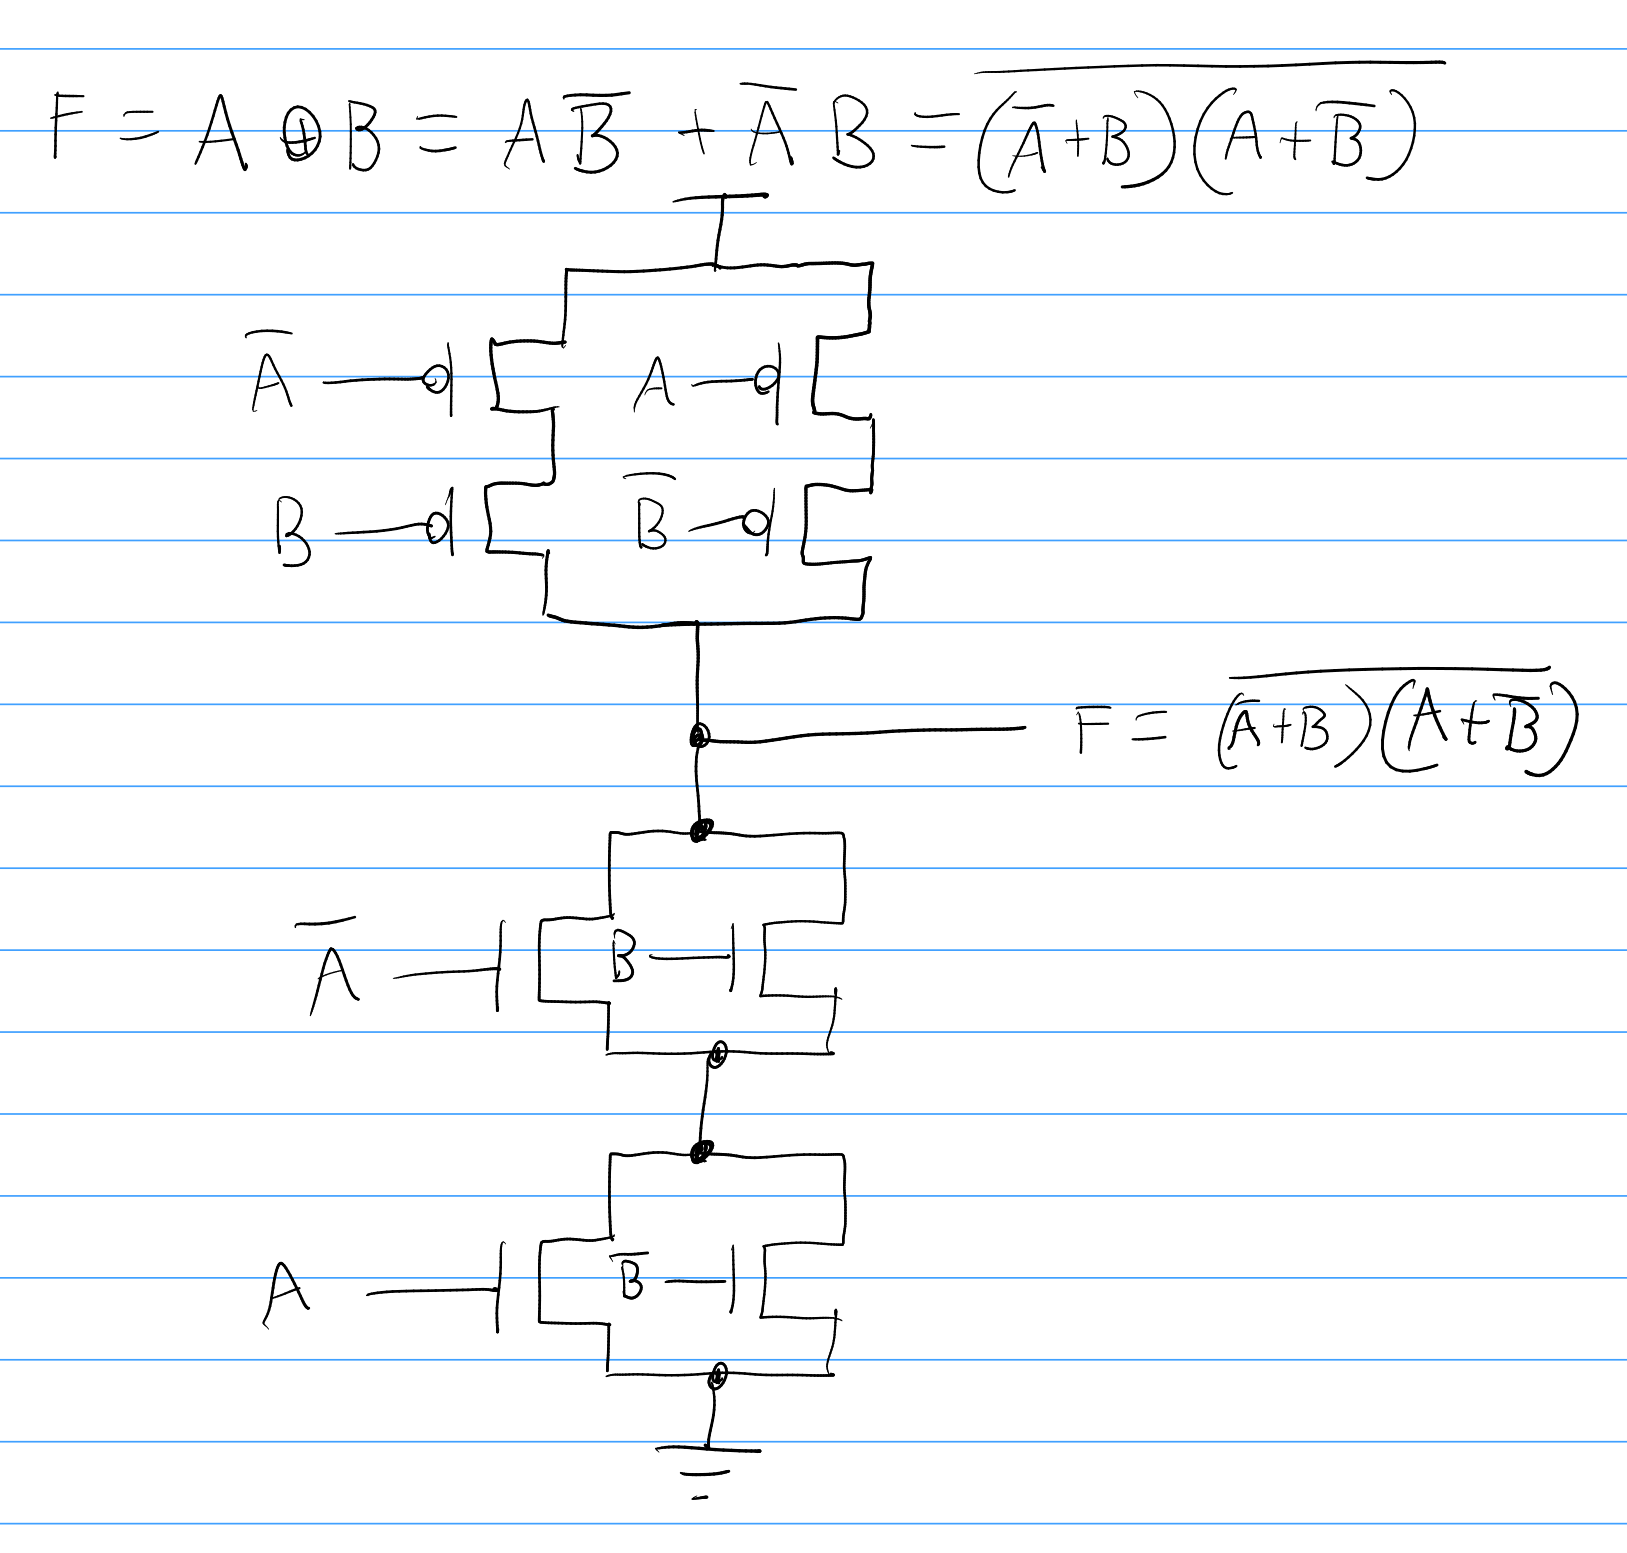
\includegraphics[width=0.7\linewidth, frame]{screenshots/schematic-sketch-1.png}
    \caption{A sketch of the PUN and PDN for implementing the XOR gate.}
    \label{fig:sketch1}
  \end{figure}

  \paragraph{}
  Since we are only given $A$ and $B$ as inputs and not $\overline{A}$ and $\overline{B}$ as well, we have to invert A and B for the inputs where $\overline{A}$ and $\overline{B}$ are necessary. This requires two inverters at the inputs, as shown in the sketch in Figure \ref{fig:sketch2}.


  \begin{figure}[H]
    \centering
    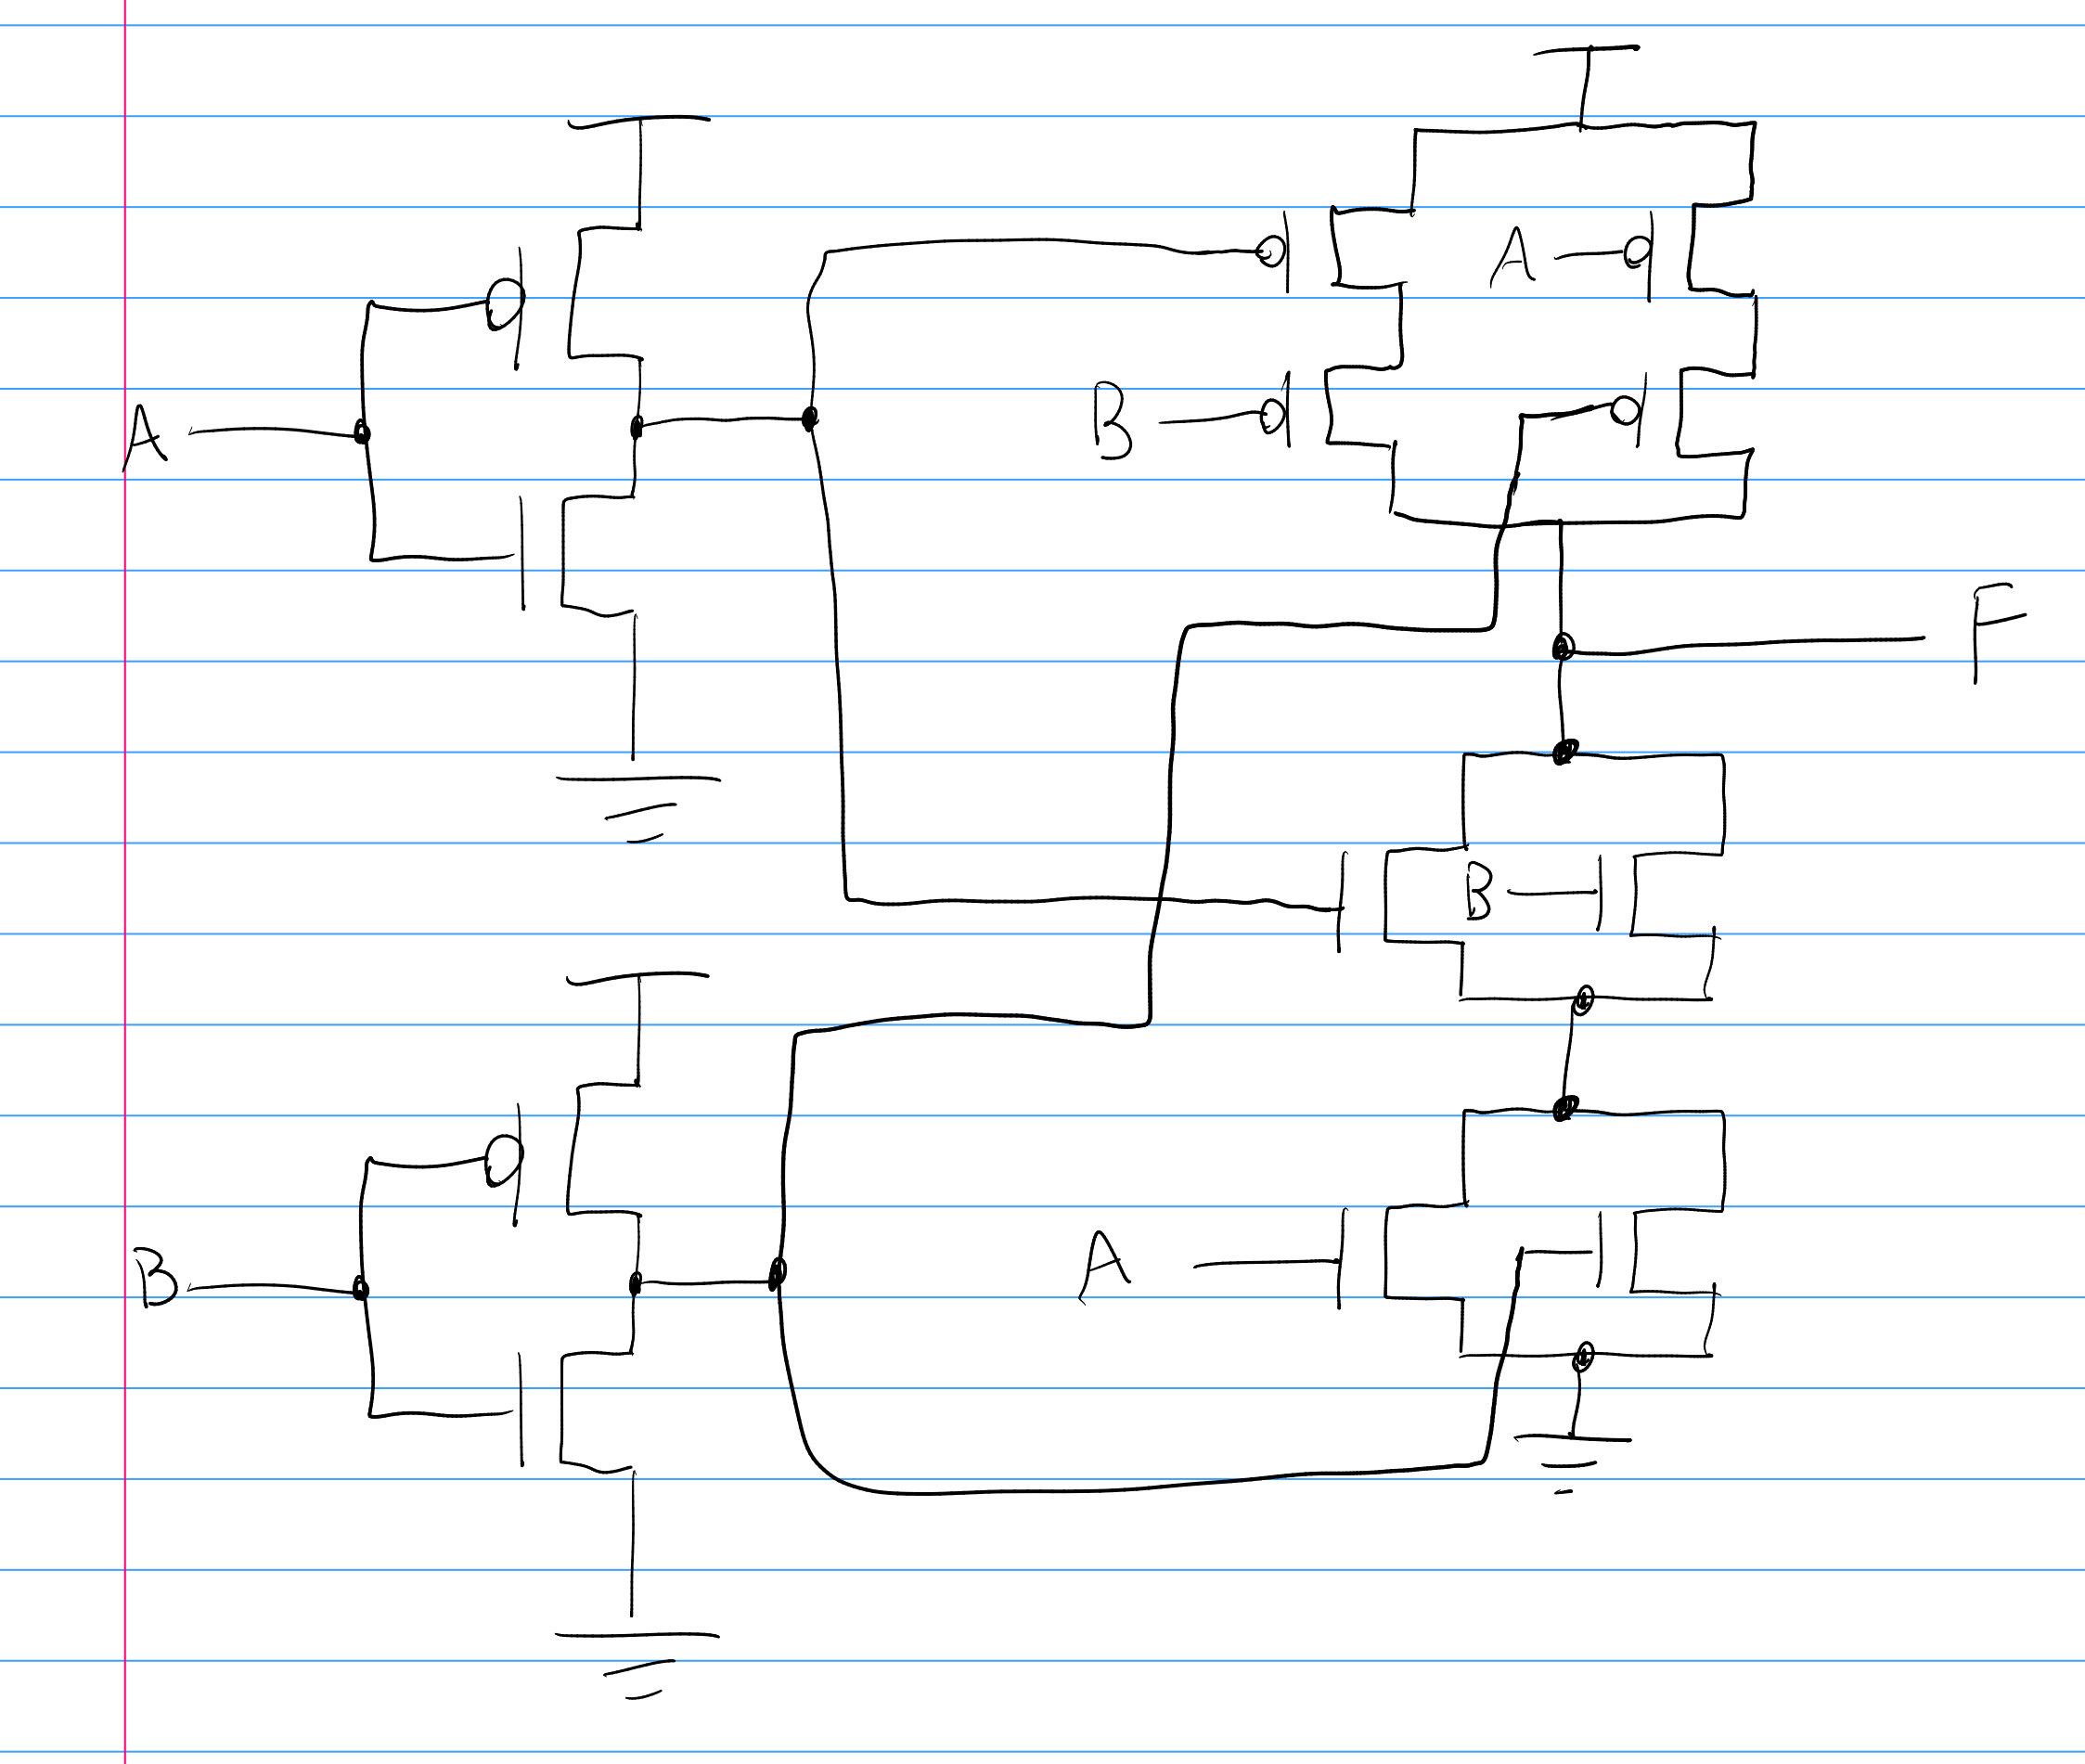
\includegraphics[width=0.7\linewidth, frame]{screenshots/schematic-sketch-2.png}
    \caption{A sketch of the XOR gate in CMOS logic.}
    \label{fig:sketch2}
  \end{figure}

\section{Schematic in Electric}

  \paragraph{}
  The sketch of the circuit was then built in the schematic design portion of Electric. The final schematic can be seen in Figure \ref{fig:schem}. The various nets that feed into the PUN and PDN are labeled to make the schematic easier to read. The transistors were initially chosen to be 8$\lambda$ wide and 2$\lambda$ long for PMOS and 4$\lambda$ wide and 2$\lambda$ because those are the dimensions that worked best for the inverter that we designed previously. However, we were told to make the PMOS transistors and NMOS transistors the same size, so I made them all 8$\lambda$ wide and 2$\lambda$.

  \begin{figure}[H]
    \centering
    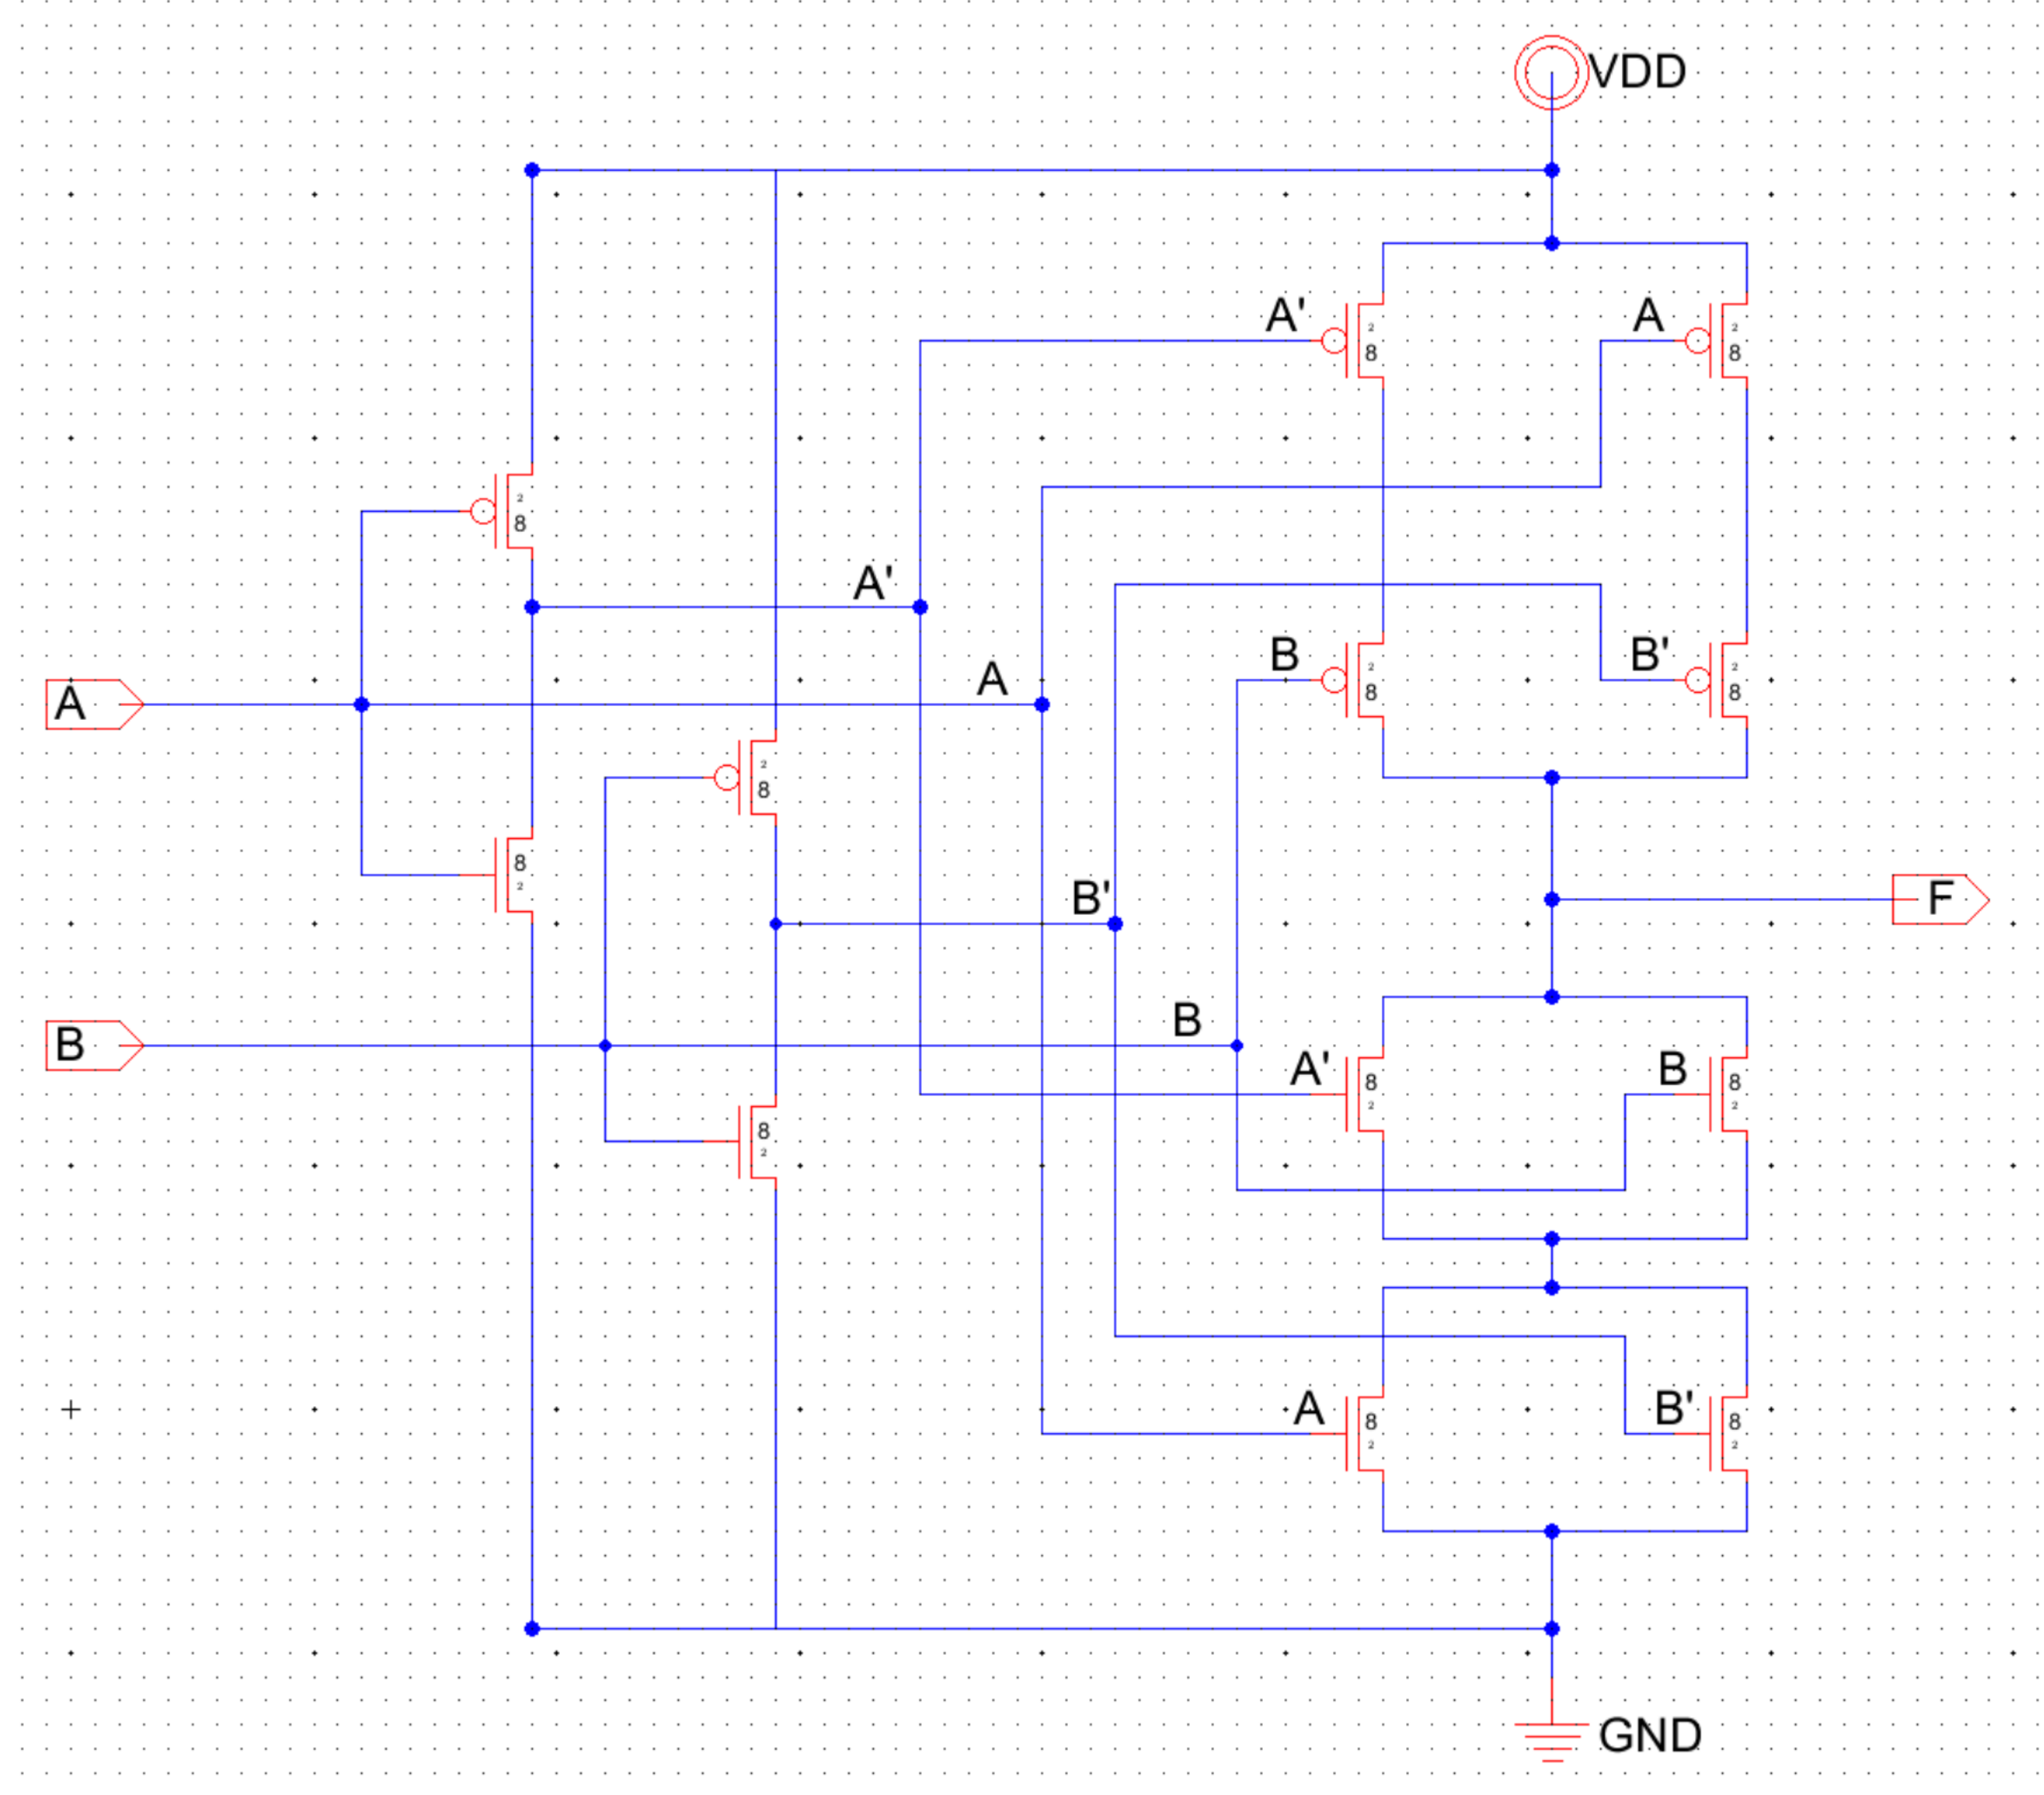
\includegraphics[width=0.9\linewidth, frame]{screenshots/schematic.png}
    \caption{The finished schematic in Electric.}
    \label{fig:schem}
  \end{figure}

  \paragraph{}
  After designing the schematic in electric, it must pass the Design Rule Check (DRC) in order to be simulated properly. The results of the DRC are shown in Figure \ref{sch-drc}.

  \begin{figure}[H]
    \centering
    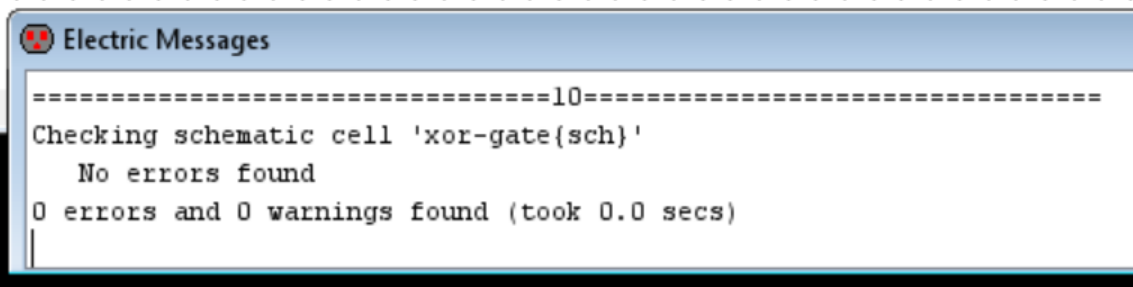
\includegraphics[width=0.9\linewidth, frame]{screenshots/schematic-drc.png}
    \caption{The DRC for the schematic shows no errors.}
    \label{fig:sch-drc}
  \end{figure}






\begin{comment}
%How to do inline code:
\paragraph{}
There is some inline code, \inlinecode{movff STATUS, STATUS\_TEMP}, in this sentence.

This formula $f(x) = x^2$ is an example of inline math.

\end{comment}


\begin{comment}
%How to do equations:

\begin{equation*}
P_{1f_m}=\int^\infty_{-\infty}G_{1f_m}(f)df=0.01\int^\infty_{-\infty}[\delta(f-2700)+\delta(f-2300)]df=0.01*(1+1)=0.02W
\end{equation*}


\end{comment}


\begin{comment}

%Here is a single figure
\begin{figure}[H]
  \centering
  \includegraphics[width=0.9\linewidth, frame]{screenshots/01.png}
  \caption{The system for this lab.}
  \label{fig:01}
\end{figure}

\end{comment}

\begin{comment}

%Here is a double figure
\begin{figure}[H]
  \centering
  \begin{subfigure}[b]{0.45\linewidth}
    \includegraphics[width=\linewidth, frame]{screenshots/02.png}
    \caption{The xyz block.}
  \end{subfigure}
  \begin{subfigure}[b]{0.45\linewidth}
    \includegraphics[width=\linewidth, frame]{screenshots/03.png}
    \caption{The abc block.}
  \end{subfigure}
  \caption{The two figures in this double figure.}
  \label{fig:02}
\end{figure}

\end{comment}


\end{document}
